% Options for packages loaded elsewhere
\PassOptionsToPackage{unicode}{hyperref}
\PassOptionsToPackage{hyphens}{url}
\PassOptionsToPackage{dvipsnames,svgnames,x11names}{xcolor}
%
\documentclass[
  letterpaper,
  DIV=11,
  numbers=noendperiod]{scrartcl}

\usepackage{amsmath,amssymb}
\usepackage{iftex}
\ifPDFTeX
  \usepackage[T1]{fontenc}
  \usepackage[utf8]{inputenc}
  \usepackage{textcomp} % provide euro and other symbols
\else % if luatex or xetex
  \usepackage{unicode-math}
  \defaultfontfeatures{Scale=MatchLowercase}
  \defaultfontfeatures[\rmfamily]{Ligatures=TeX,Scale=1}
\fi
\usepackage{lmodern}
\ifPDFTeX\else  
    % xetex/luatex font selection
\fi
% Use upquote if available, for straight quotes in verbatim environments
\IfFileExists{upquote.sty}{\usepackage{upquote}}{}
\IfFileExists{microtype.sty}{% use microtype if available
  \usepackage[]{microtype}
  \UseMicrotypeSet[protrusion]{basicmath} % disable protrusion for tt fonts
}{}
\makeatletter
\@ifundefined{KOMAClassName}{% if non-KOMA class
  \IfFileExists{parskip.sty}{%
    \usepackage{parskip}
  }{% else
    \setlength{\parindent}{0pt}
    \setlength{\parskip}{6pt plus 2pt minus 1pt}}
}{% if KOMA class
  \KOMAoptions{parskip=half}}
\makeatother
\usepackage{xcolor}
\setlength{\emergencystretch}{3em} % prevent overfull lines
\setcounter{secnumdepth}{-\maxdimen} % remove section numbering
% Make \paragraph and \subparagraph free-standing
\ifx\paragraph\undefined\else
  \let\oldparagraph\paragraph
  \renewcommand{\paragraph}[1]{\oldparagraph{#1}\mbox{}}
\fi
\ifx\subparagraph\undefined\else
  \let\oldsubparagraph\subparagraph
  \renewcommand{\subparagraph}[1]{\oldsubparagraph{#1}\mbox{}}
\fi


\providecommand{\tightlist}{%
  \setlength{\itemsep}{0pt}\setlength{\parskip}{0pt}}\usepackage{longtable,booktabs,array}
\usepackage{calc} % for calculating minipage widths
% Correct order of tables after \paragraph or \subparagraph
\usepackage{etoolbox}
\makeatletter
\patchcmd\longtable{\par}{\if@noskipsec\mbox{}\fi\par}{}{}
\makeatother
% Allow footnotes in longtable head/foot
\IfFileExists{footnotehyper.sty}{\usepackage{footnotehyper}}{\usepackage{footnote}}
\makesavenoteenv{longtable}
\usepackage{graphicx}
\makeatletter
\def\maxwidth{\ifdim\Gin@nat@width>\linewidth\linewidth\else\Gin@nat@width\fi}
\def\maxheight{\ifdim\Gin@nat@height>\textheight\textheight\else\Gin@nat@height\fi}
\makeatother
% Scale images if necessary, so that they will not overflow the page
% margins by default, and it is still possible to overwrite the defaults
% using explicit options in \includegraphics[width, height, ...]{}
\setkeys{Gin}{width=\maxwidth,height=\maxheight,keepaspectratio}
% Set default figure placement to htbp
\makeatletter
\def\fps@figure{htbp}
\makeatother
% definitions for citeproc citations
\NewDocumentCommand\citeproctext{}{}
\NewDocumentCommand\citeproc{mm}{%
  \begingroup\def\citeproctext{#2}\cite{#1}\endgroup}
\makeatletter
 % allow citations to break across lines
 \let\@cite@ofmt\@firstofone
 % avoid brackets around text for \cite:
 \def\@biblabel#1{}
 \def\@cite#1#2{{#1\if@tempswa , #2\fi}}
\makeatother
\newlength{\cslhangindent}
\setlength{\cslhangindent}{1.5em}
\newlength{\csllabelwidth}
\setlength{\csllabelwidth}{3em}
\newenvironment{CSLReferences}[2] % #1 hanging-indent, #2 entry-spacing
 {\begin{list}{}{%
  \setlength{\itemindent}{0pt}
  \setlength{\leftmargin}{0pt}
  \setlength{\parsep}{0pt}
  % turn on hanging indent if param 1 is 1
  \ifodd #1
   \setlength{\leftmargin}{\cslhangindent}
   \setlength{\itemindent}{-1\cslhangindent}
  \fi
  % set entry spacing
  \setlength{\itemsep}{#2\baselineskip}}}
 {\end{list}}
\usepackage{calc}
\newcommand{\CSLBlock}[1]{\hfill\break\parbox[t]{\linewidth}{\strut\ignorespaces#1\strut}}
\newcommand{\CSLLeftMargin}[1]{\parbox[t]{\csllabelwidth}{\strut#1\strut}}
\newcommand{\CSLRightInline}[1]{\parbox[t]{\linewidth - \csllabelwidth}{\strut#1\strut}}
\newcommand{\CSLIndent}[1]{\hspace{\cslhangindent}#1}

\usepackage{float}
\usepackage{tabularray}
\usepackage[normalem]{ulem}
\usepackage{graphicx}
\UseTblrLibrary{booktabs}
\UseTblrLibrary{rotating}
\UseTblrLibrary{siunitx}
\NewTableCommand{\tinytableDefineColor}[3]{\definecolor{#1}{#2}{#3}}
\newcommand{\tinytableTabularrayUnderline}[1]{\underline{#1}}
\newcommand{\tinytableTabularrayStrikeout}[1]{\sout{#1}}
\KOMAoption{captions}{tableheading}
\makeatletter
\@ifpackageloaded{caption}{}{\usepackage{caption}}
\AtBeginDocument{%
\ifdefined\contentsname
  \renewcommand*\contentsname{Table of contents}
\else
  \newcommand\contentsname{Table of contents}
\fi
\ifdefined\listfigurename
  \renewcommand*\listfigurename{List of Figures}
\else
  \newcommand\listfigurename{List of Figures}
\fi
\ifdefined\listtablename
  \renewcommand*\listtablename{List of Tables}
\else
  \newcommand\listtablename{List of Tables}
\fi
\ifdefined\figurename
  \renewcommand*\figurename{Figure}
\else
  \newcommand\figurename{Figure}
\fi
\ifdefined\tablename
  \renewcommand*\tablename{Table}
\else
  \newcommand\tablename{Table}
\fi
}
\@ifpackageloaded{float}{}{\usepackage{float}}
\floatstyle{ruled}
\@ifundefined{c@chapter}{\newfloat{codelisting}{h}{lop}}{\newfloat{codelisting}{h}{lop}[chapter]}
\floatname{codelisting}{Listing}
\newcommand*\listoflistings{\listof{codelisting}{List of Listings}}
\makeatother
\makeatletter
\makeatother
\makeatletter
\@ifpackageloaded{caption}{}{\usepackage{caption}}
\@ifpackageloaded{subcaption}{}{\usepackage{subcaption}}
\makeatother
\ifLuaTeX
  \usepackage{selnolig}  % disable illegal ligatures
\fi
\usepackage{bookmark}

\IfFileExists{xurl.sty}{\usepackage{xurl}}{} % add URL line breaks if available
\urlstyle{same} % disable monospaced font for URLs
\hypersetup{
  pdftitle={Public Internet Correlation between Population Density or Schools},
  colorlinks=true,
  linkcolor={blue},
  filecolor={Maroon},
  citecolor={Blue},
  urlcolor={Blue},
  pdfcreator={LaTeX via pandoc}}

\title{Public Internet Correlation between Population Density or
Schools}
\usepackage{etoolbox}
\makeatletter
\providecommand{\subtitle}[1]{% add subtitle to \maketitle
  \apptocmd{\@title}{\par {\large #1 \par}}{}{}
}
\makeatother
\subtitle{DSAN 6750 / PPOL 6805: GIS for Spatial Data Science}
\author{Gabriel Soto}
\date{}

\begin{document}
\maketitle

\subsection{Introduction}\label{introduction}

Do public schools get better access to public internet? This research
analyses whether public schools in Panama, get access to public internet
via access points - Google Satellite - Migration Panama

\begin{itemize}
\tightlist
\item
  meter data temporal de uso de datos por access points
\item
  agregar datos de cantidad de estudiantes por distrito
  https://www.inec.gob.pa/archivos/P030194820231213142523Cuadro\%2021.pdf
\item
  agregar un indice normalizado (ya que el numero es muy chiquito) de la
  cantidad de casas sin internet
  https://www.inec.gob.pa/archivos/P0705547520240202111515Cuadro\%201.pdf
\end{itemize}

Future: - indicadores socioeconomicos a nivel de distrito
https://www.inec.gob.pa/archivos/P0579518620240202083001Cuadro\%204.pdf

dijo:

\begin{quote}
It's the remoteness of Oyala that makes it so appealing to President
Obiang. In a rare interview he described how rebels had recently plotted
a seaborne assault on his palace in the current capital, Malabo. `We
need a secure place for my government and for future governments. That's
why we have created Oyala, to guarantee the government of Equatorial
Guinea.' (\citeproc{ref-sackur_equatorial_2012}{Sackur 2012})
\end{quote}

This case is far from exceptional, as an even more recent
\emph{Washington Post} article points out with respect to Myanmar's
decision to move its capital from Yangon to Naypyidaw:

\begin{quote}
Analysts have described the decision as motivated by a desire to secure
the military's seat of power from any threat of protests or invasions.
(\citeproc{ref-berger_myanmars_2021}{Berger 2021})
\end{quote}

Most of these studies, however, are based on observations of
\textbf{conflict events}. In this study, we study the more fundamental
variable of a capital's distance from the \textbf{population centroid}
of the country.

\subsection{Literature Review}\label{literature-review}

Campante, Do, and Guimaraes (\citeproc{ref-campante_capital_2019}{2019})
analyzes the relationship between the location of a \textbf{capital
city} and the degree of conflict and misgovernance in a given country.
Their two key findings are that:

\begin{quote}
Conflict is more likely to emerge (and dislodge incumbents) closer to
the capital
\end{quote}

and

\begin{quote}
Isolated capitals are associated with misgovernance.
\end{quote}

This first finding is illustrated in \textbf{?@fig-conflict-dist}

\subsection{Exploratory Data Analysis
(EDA)}\label{exploratory-data-analysis-eda}

Below we display two tables for both ** Districts and at the Province
level ** showing relevant indicators such as: - Numbers of schools -
Numbers of Access Points - Population - Access Points per School Ratio -
Access Points per 1000 people Ratio

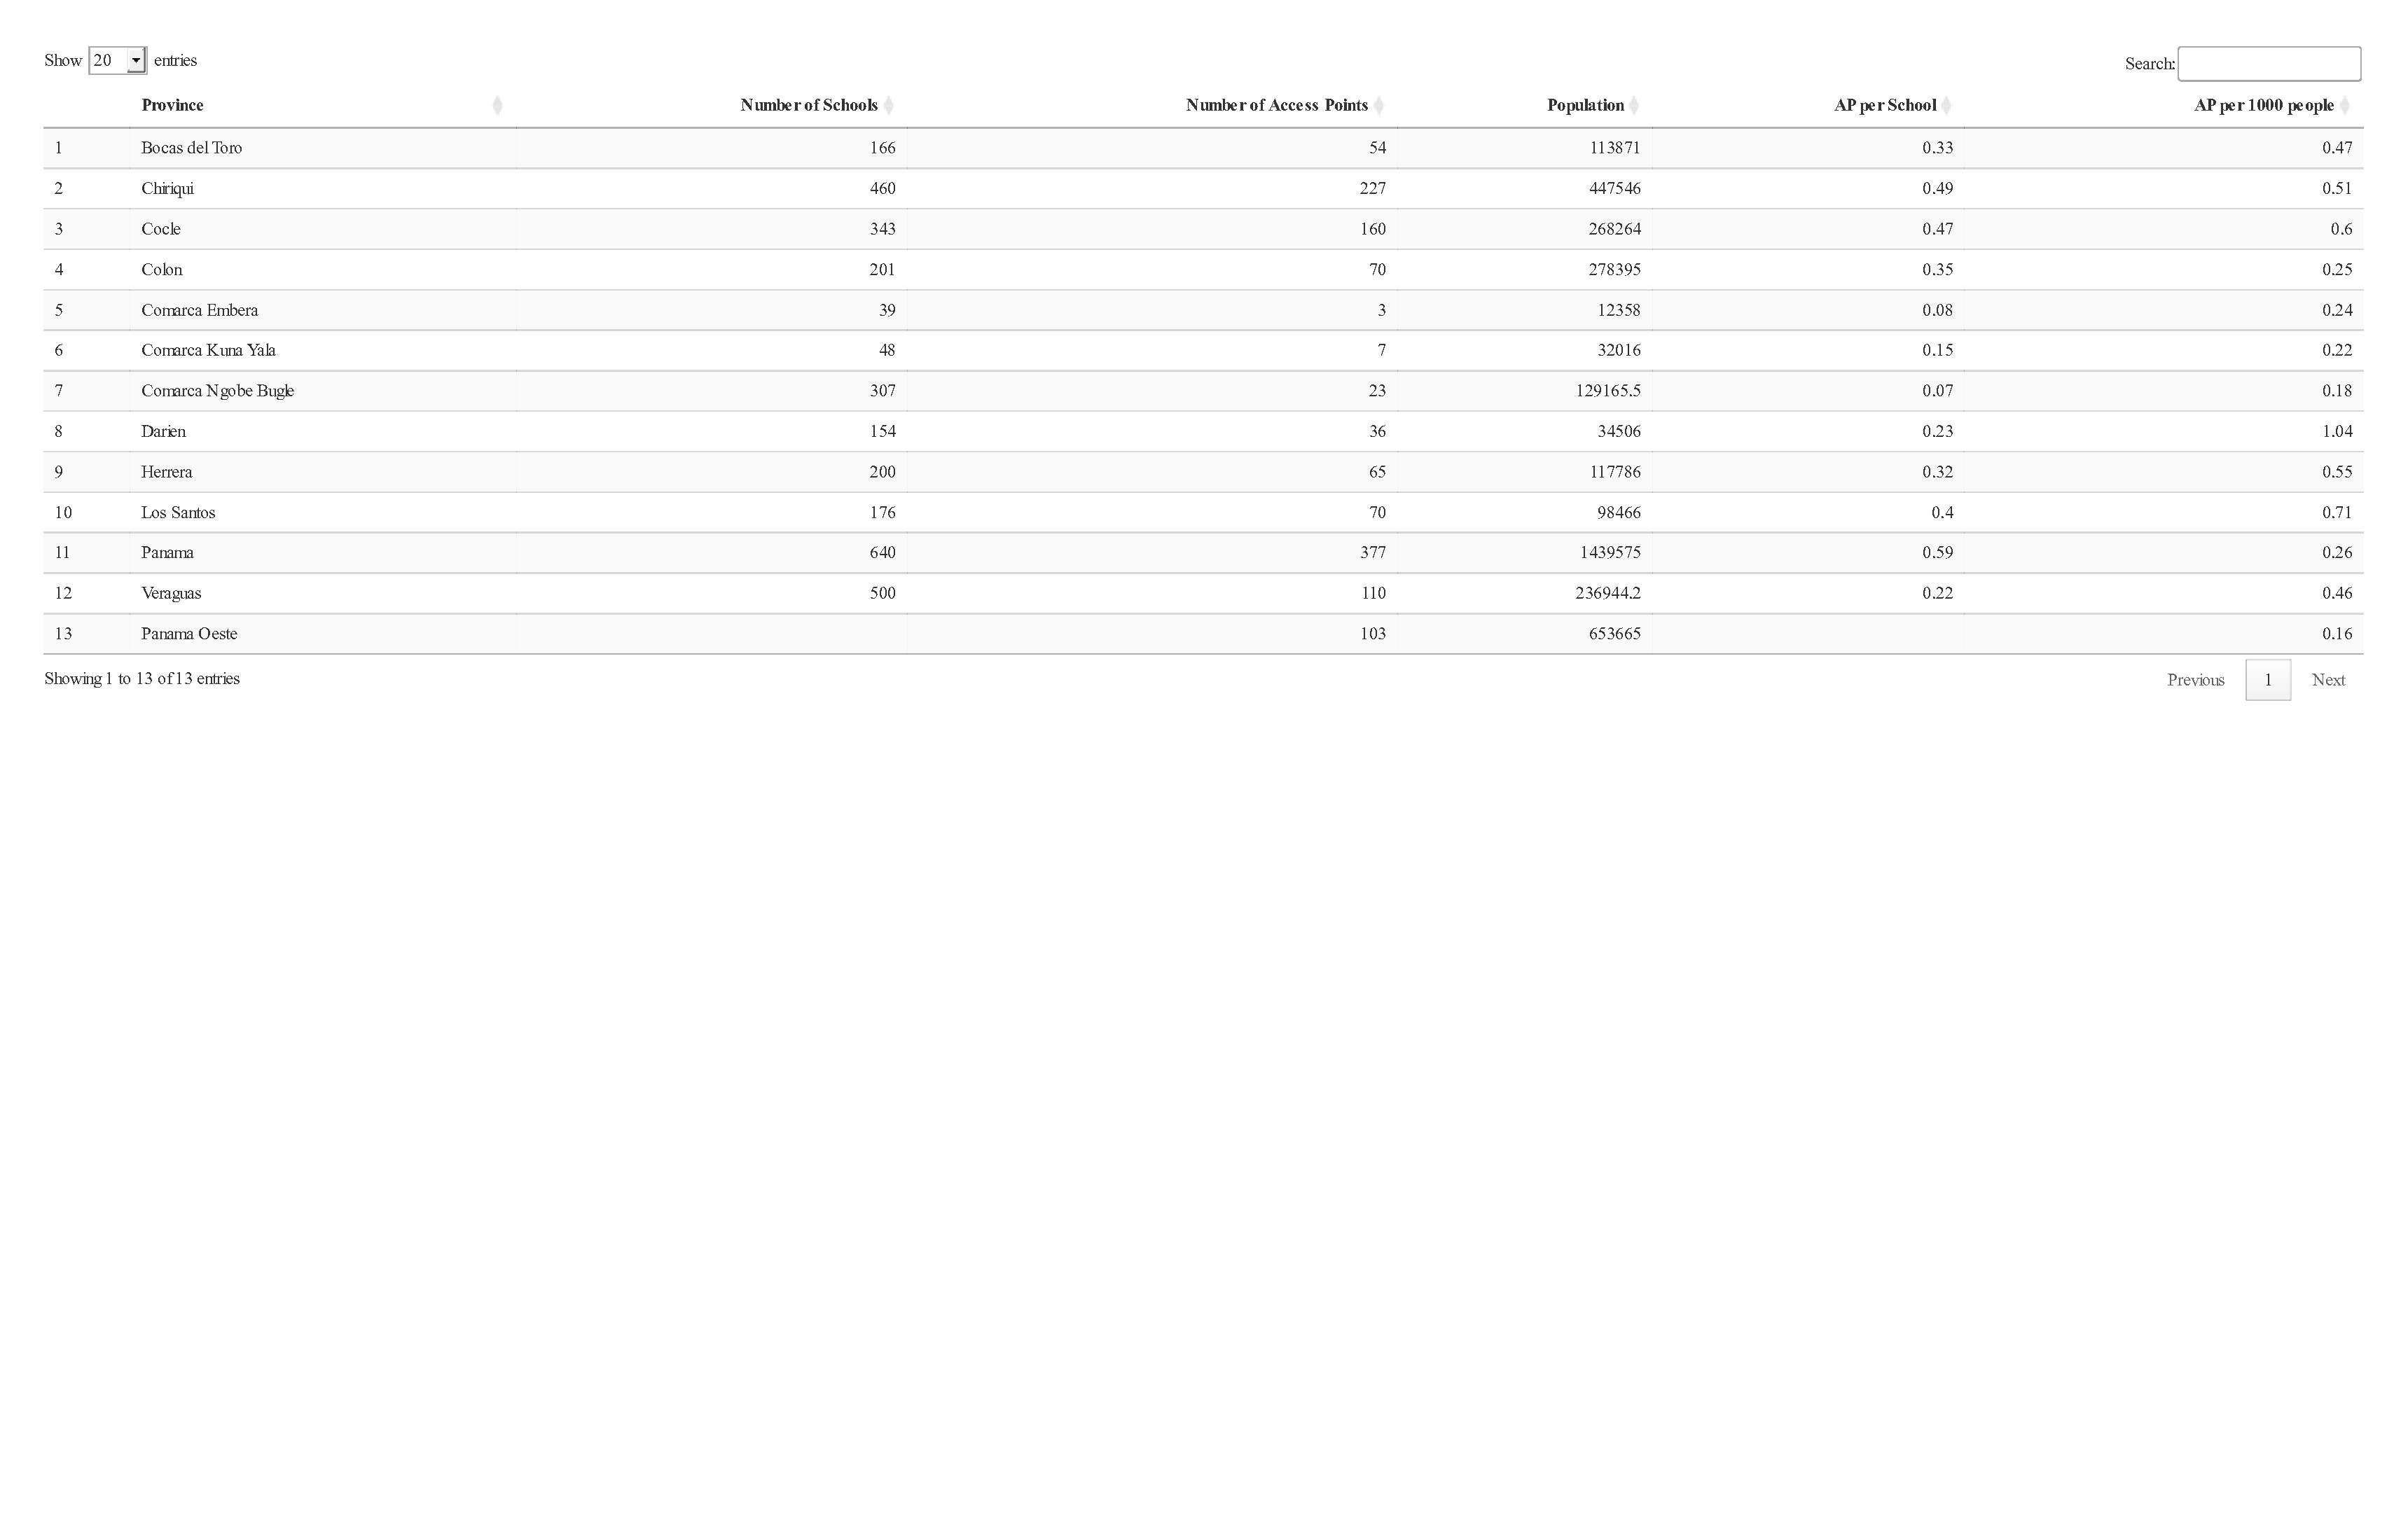
\includegraphics{index_files/figure-pdf/exploratoy-data-analysis-1.pdf}

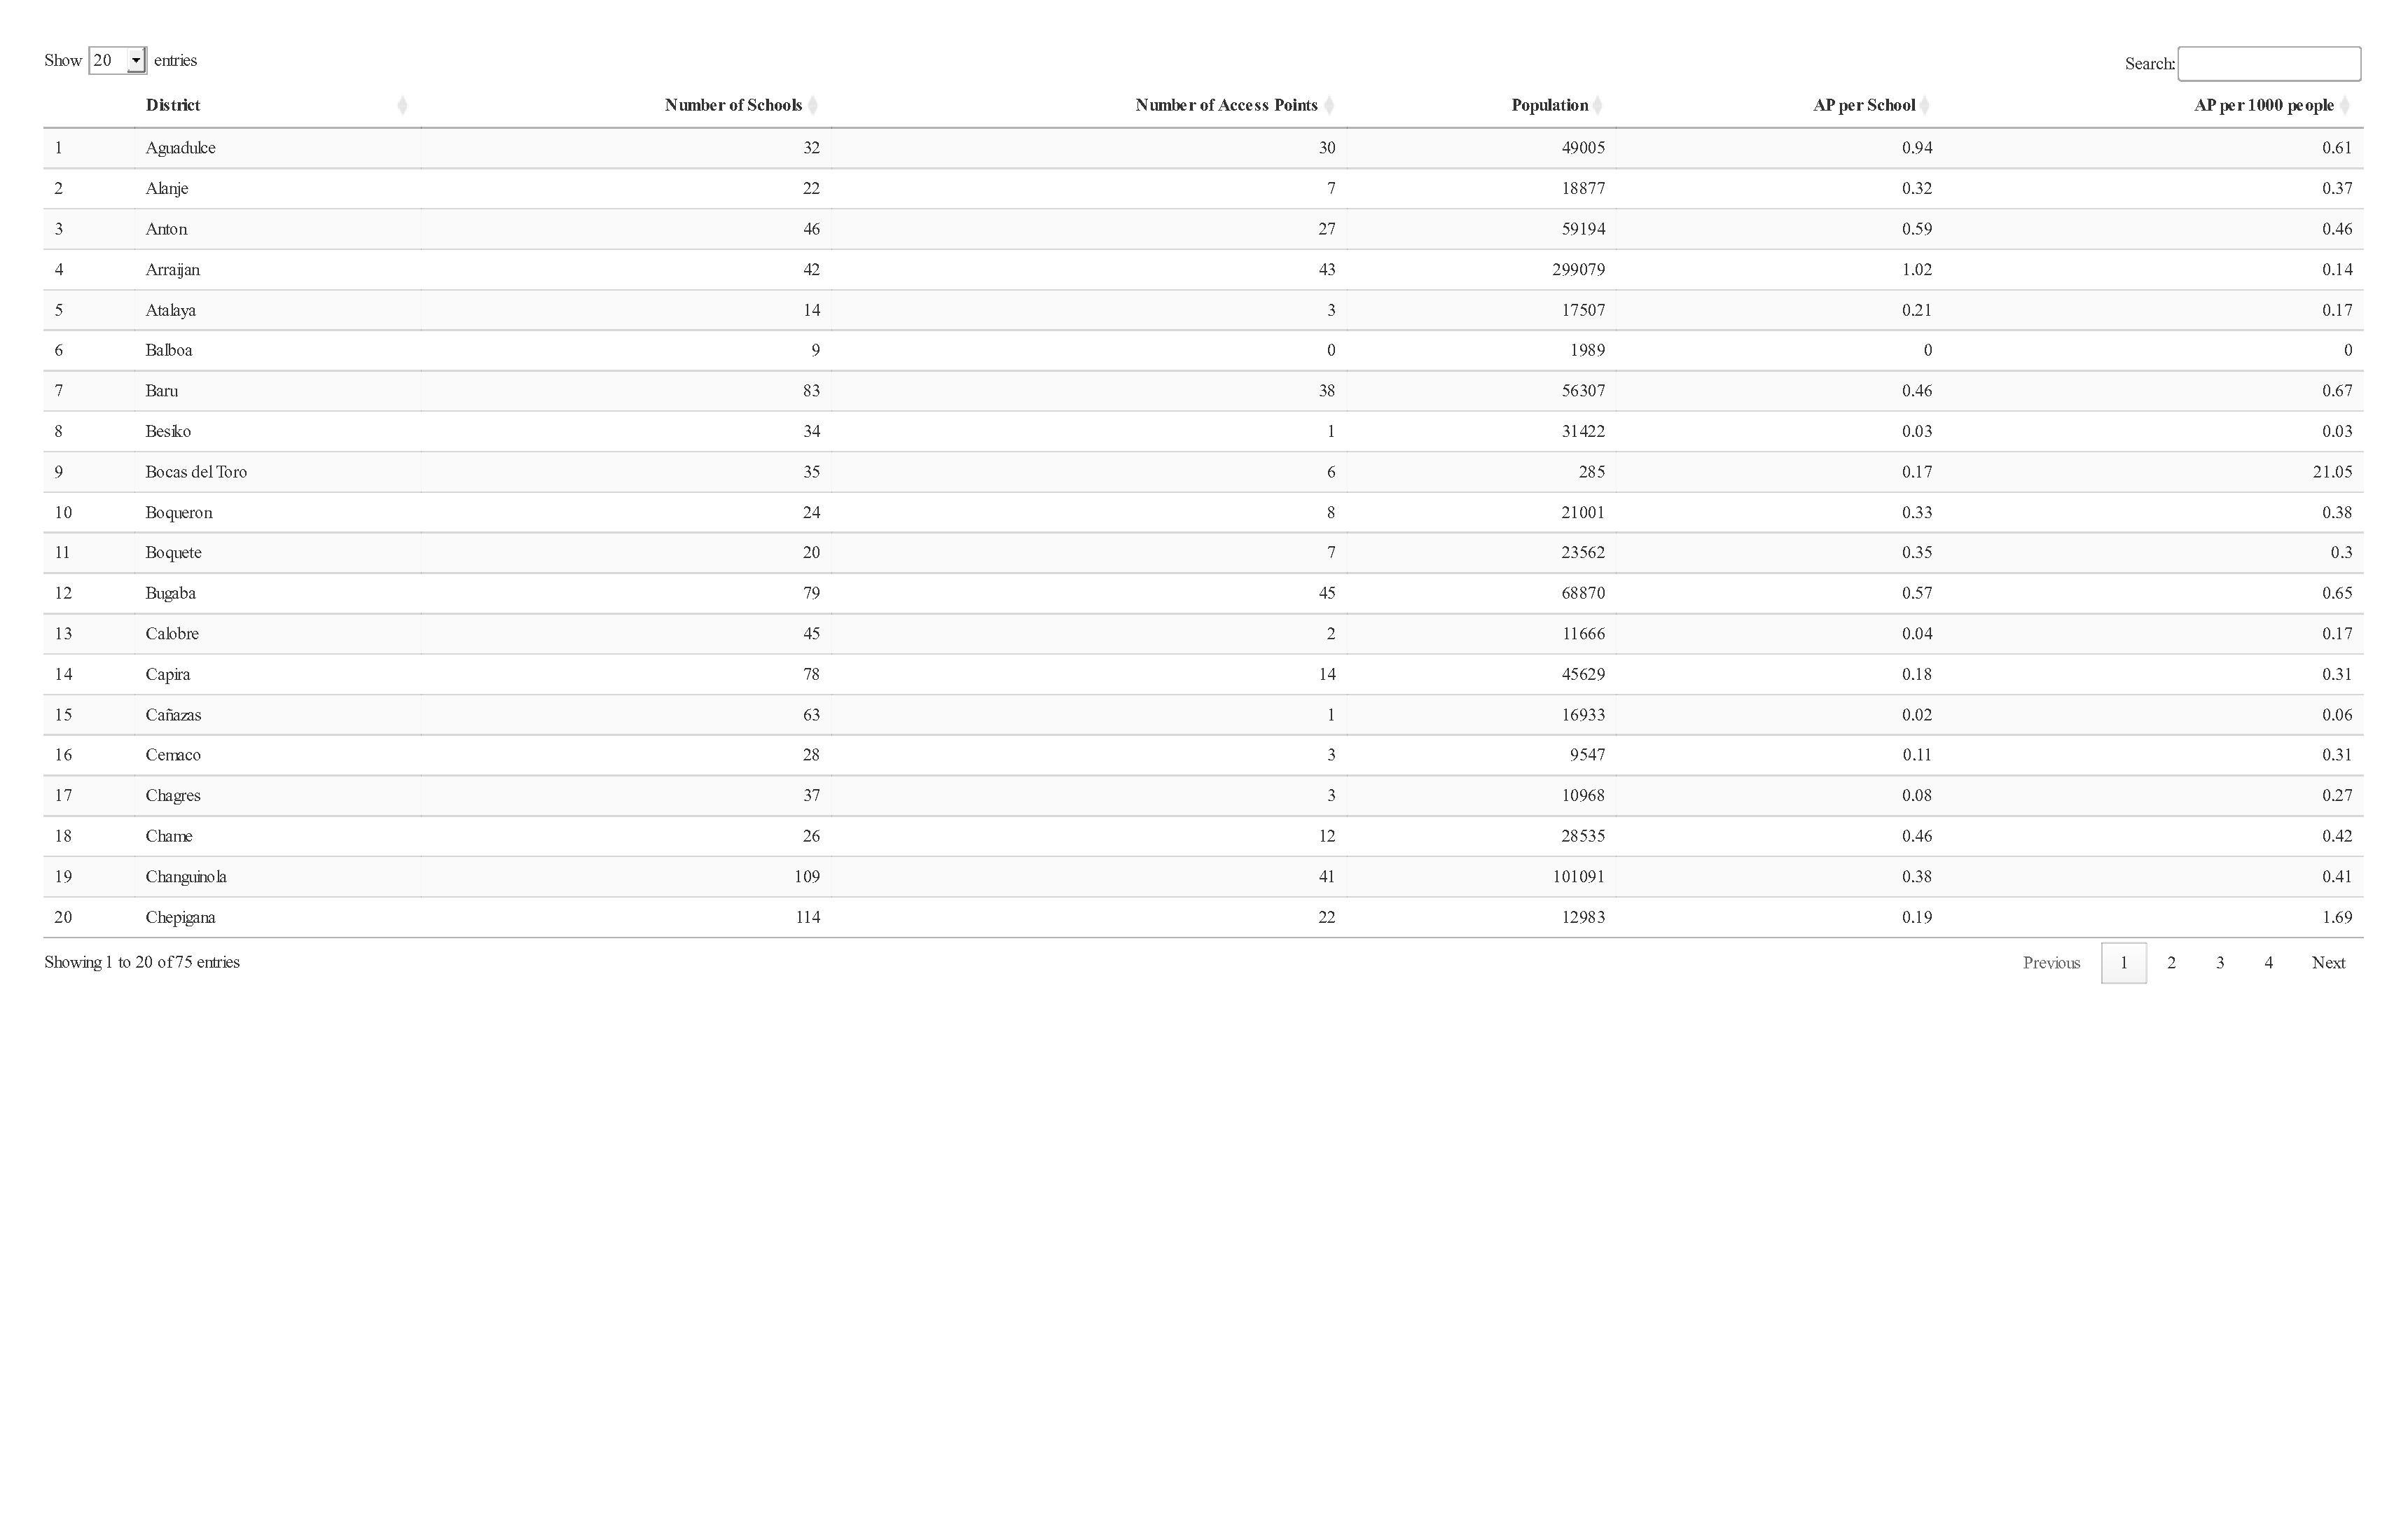
\includegraphics{index_files/figure-pdf/exploratoy-data-analysis-2.pdf}

We can see from the above tables, that Districts that house cities, are
the ones with higher amounts of access points. We see the same behavior
with the Provinces, specially with main cities such as Panama, Veraguas
and Chiriqui. Most of these studies, however, are based on observations
of \textbf{conflict events}. In this study, we study the more
fundamental variable of a capital's distance from the \textbf{population
centroid} of the country.

\textbf{Correlations between Population, Schools and Access Points}

Below I show 2 plots, where on the left we see the relationship between
Access points and Population and on the right, we see the relationship
between Access Point-School ratio with the Population.

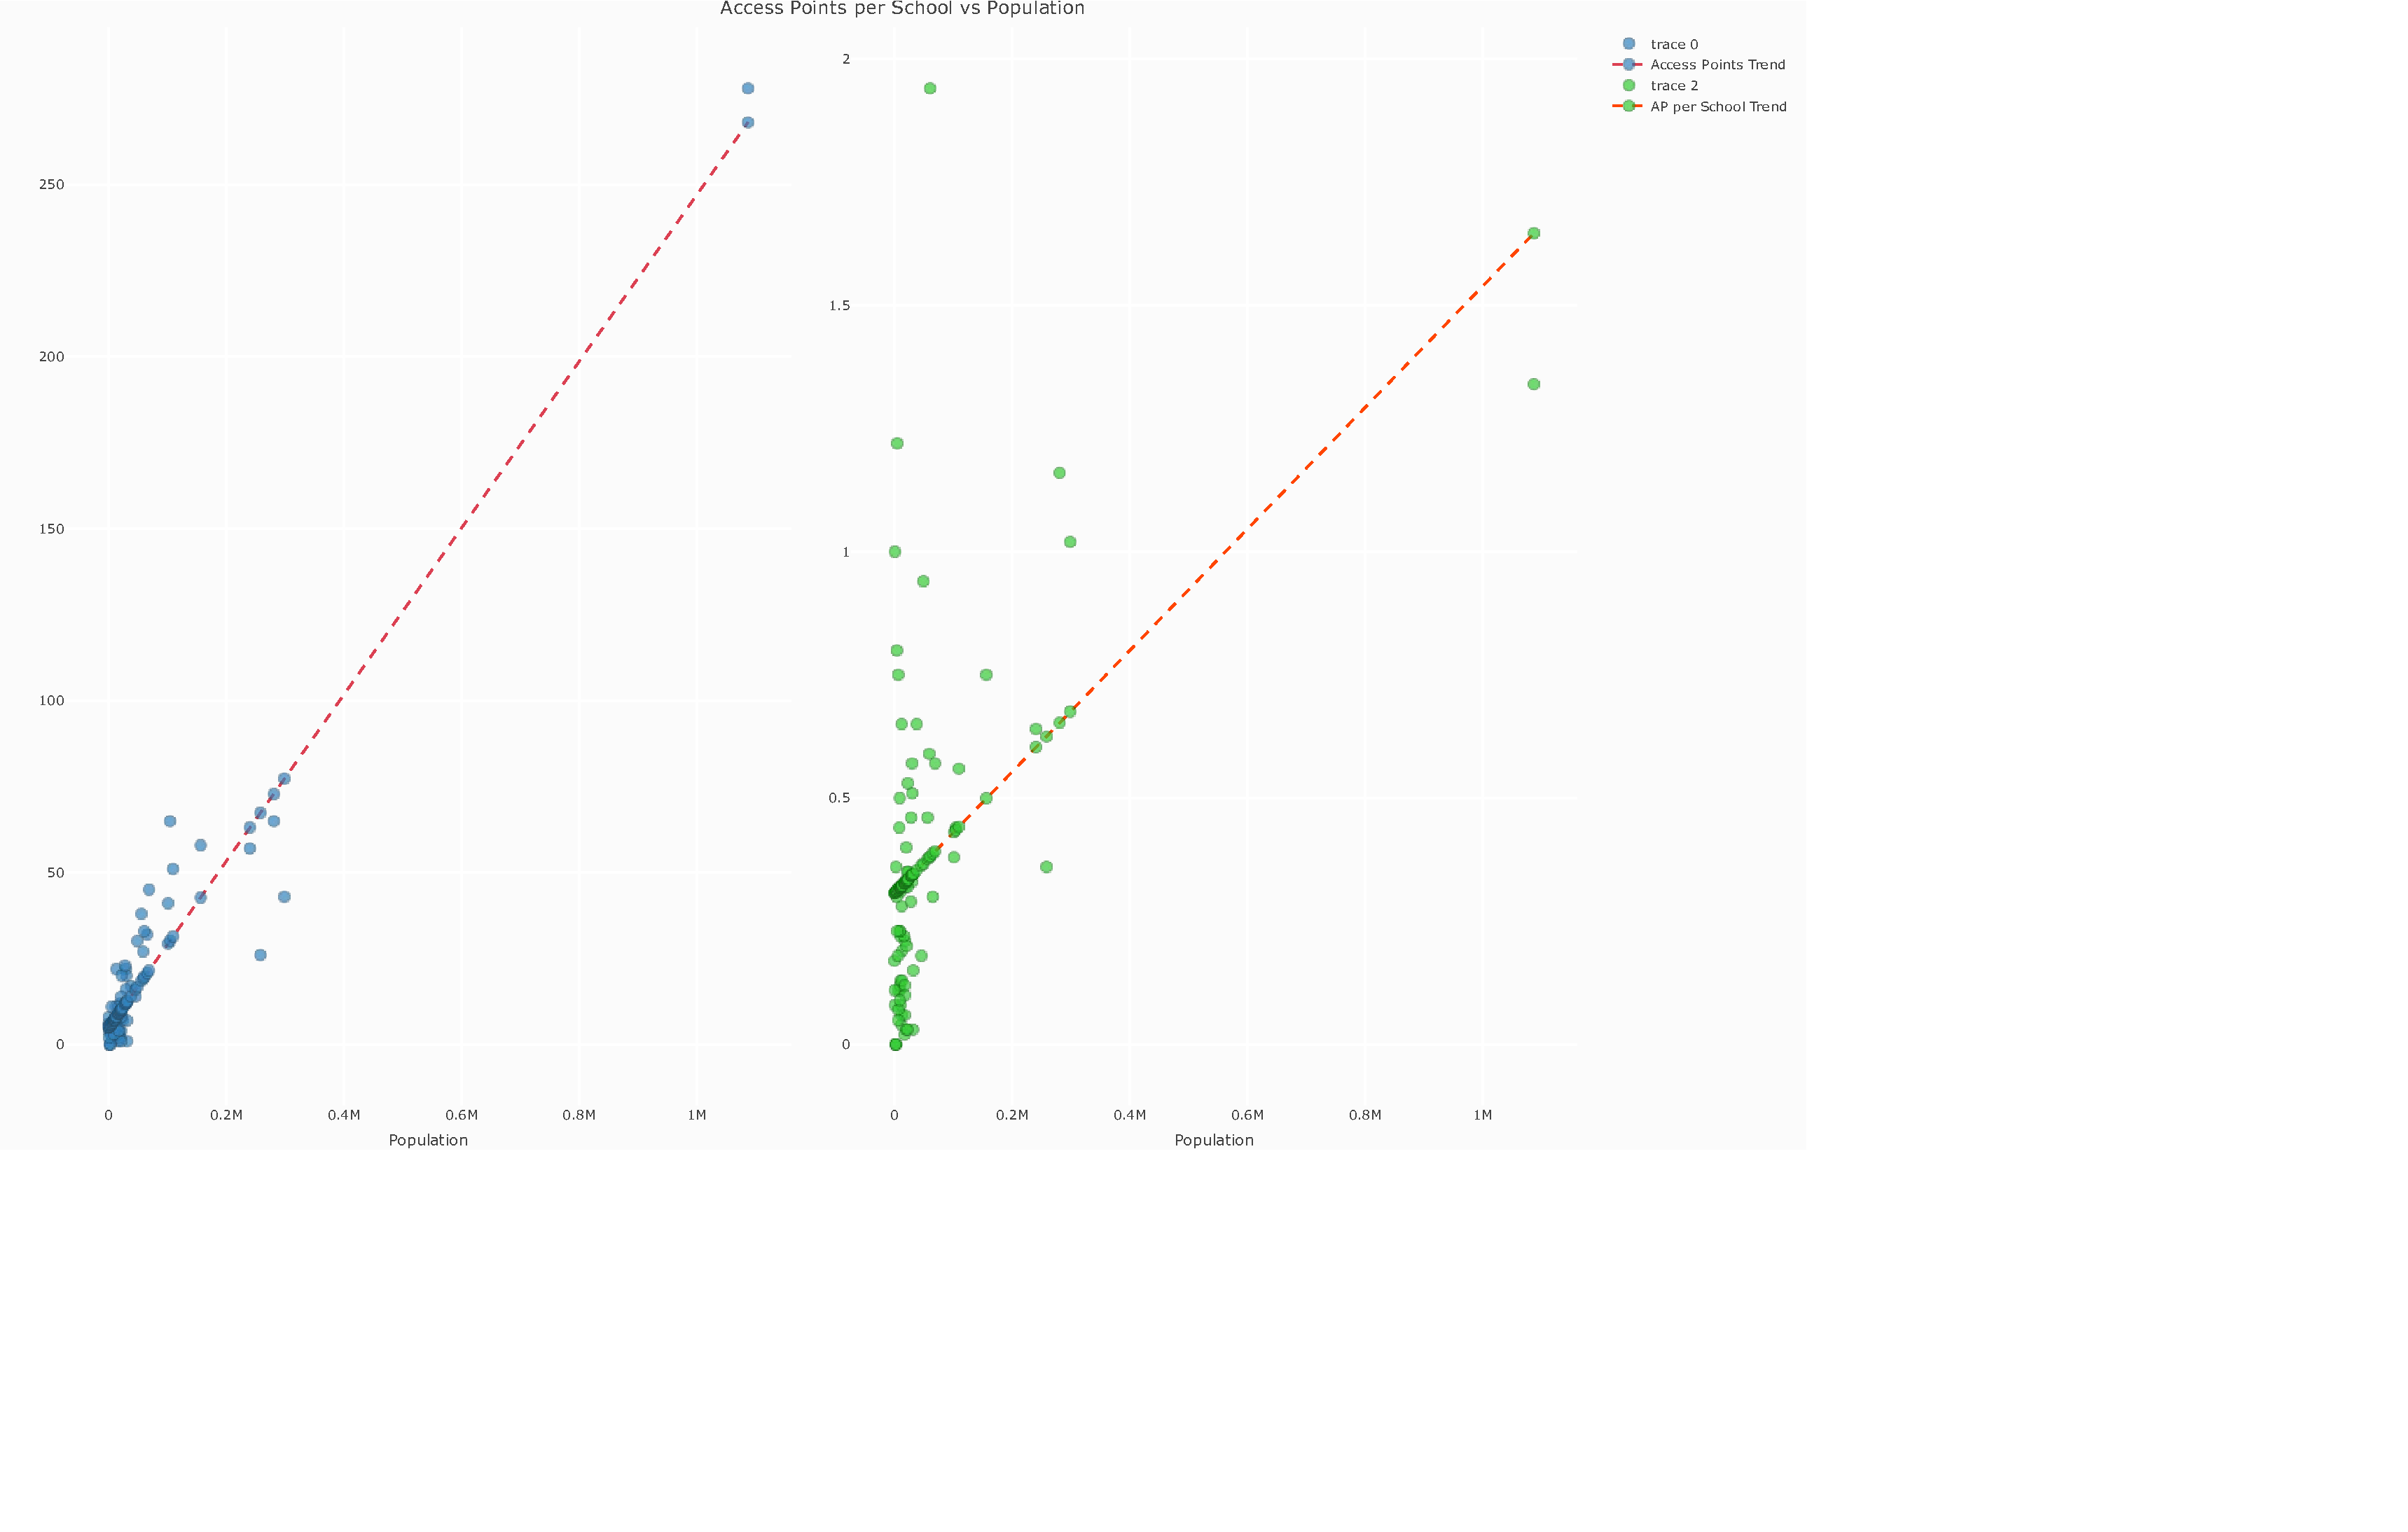
\includegraphics{index_files/figure-pdf/summary-plots-1.pdf}

\textbf{Statistical Regression of Access Points on Population}

I have run 2 statistical regression models, where I regress Access
Points on Population and Access Points both on Population and Schools.
Adding schools improves the model's explanatory power (R² increased by
2.6\%). Both population and schools are significant predictors as we can
see in the below tables. We can see that for each additional school, we
expect 0.216 more access points, holding population constant

\begin{table}
\centering
\begin{talltblr}[         %% tabularray outer open
caption={Regression Results: Access Points, Population, and Schools},
note{}={+ p \num{< 0.1}, * p \num{< 0.05}, ** p \num{< 0.01}, *** p \num{< 0.001}},
]                     %% tabularray outer close
{                     %% tabularray inner open
colspec={Q[]Q[]Q[]},
column{2,3}={}{halign=c,},
column{1}={}{halign=l,},
hline{8}={1,2,3}{solid, black, 0.05em},
}                     %% tabularray inner close
\toprule
& Model 1 & Model 2 \\ \midrule %% TinyTableHeader
Intercept  & \num{4.874}*** & \num{-2.568}   \\
& (\num{1.302})  & (\num{1.772})  \\
Population & \num{0.000}*** & \num{0.000}*** \\
& (\num{0.000})  & (\num{0.000})  \\
Schools    &                 & \num{0.216}*** \\
&                 & (\num{0.040})  \\
Num.Obs.   & \num{75}       & \num{75}       \\
R2         & \num{0.909}    & \num{0.935}    \\
R2 Adj.    & \num{0.907}    & \num{0.933}    \\
\bottomrule
\end{talltblr}
\end{table}

\subsection{Geospatial Analysis}\label{geospatial-analysis}

\textbf{Access Points Map}

Let's explore how access points are distributed along the country. As
validated above, the districts with the highest amount of access points
are those located around Panama City (459 approx), Santiago with 198 and
Boquete with approximately 118 access points. Interestingly we can
detect that probably these clusters, do not follow a random location.

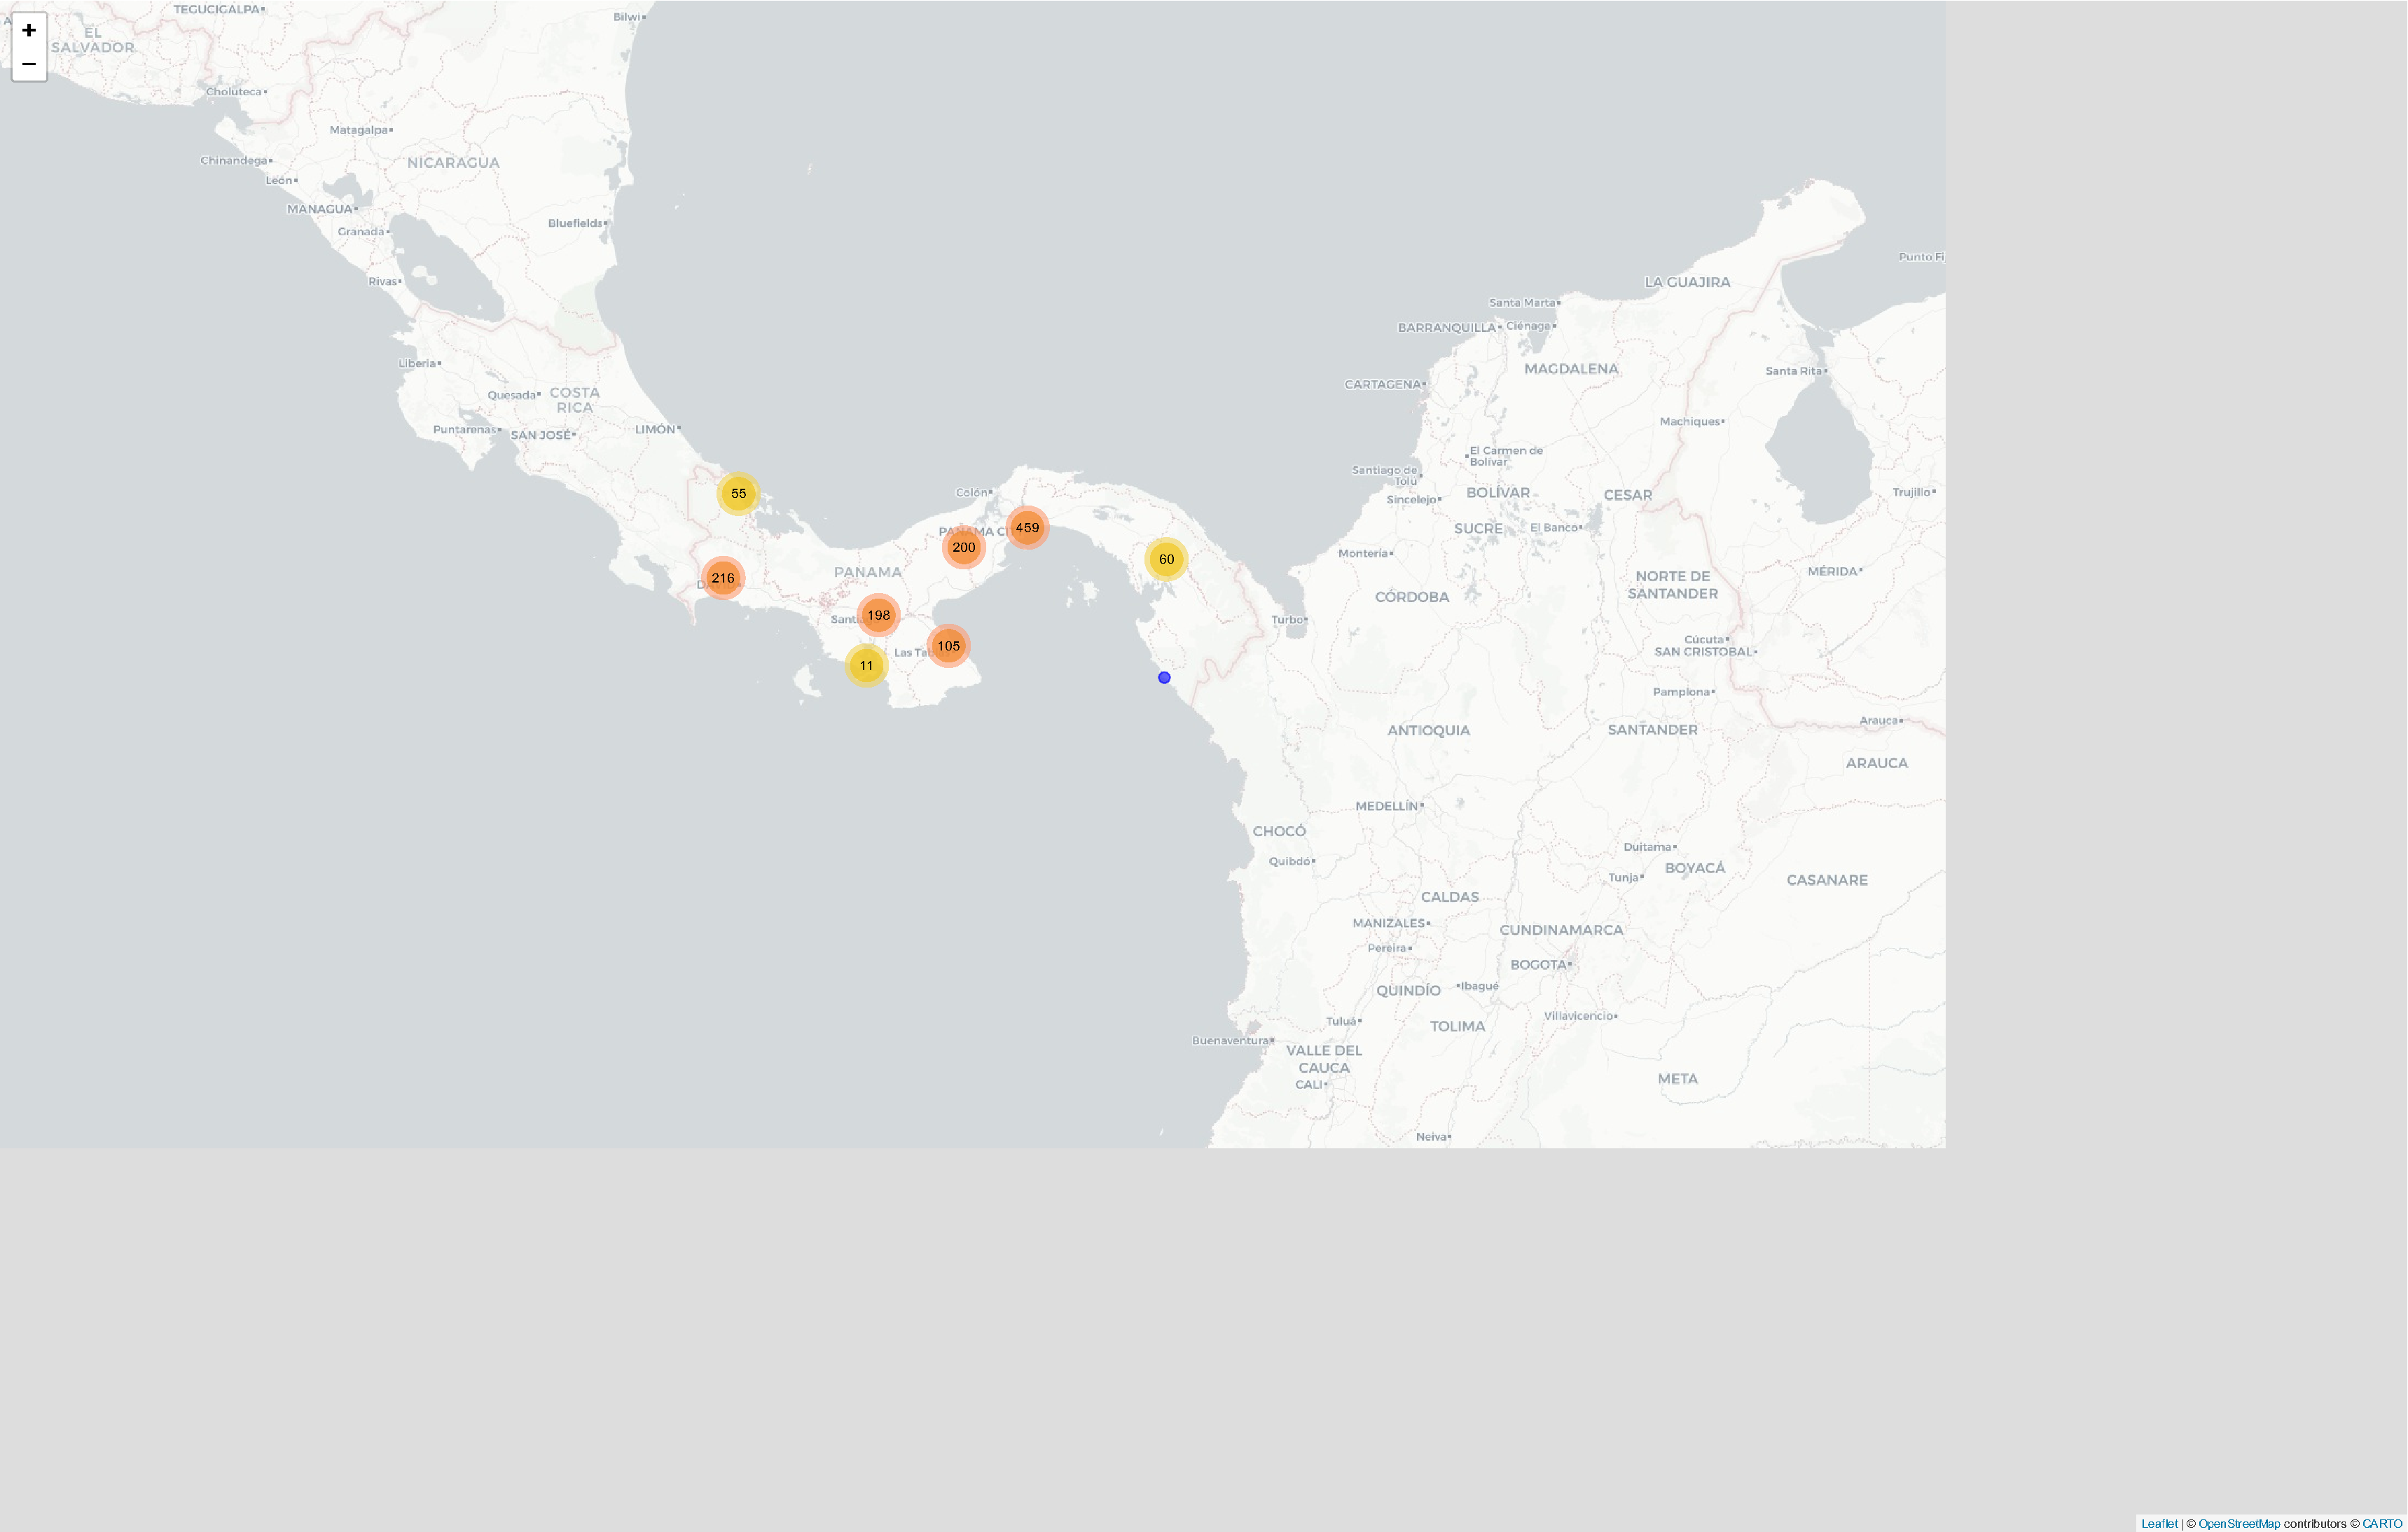
\includegraphics{index_files/figure-pdf/access-points-map-1.pdf}

\textbf{Access Points Density per District Map}

Now let's explore how different access points density is within
districts. With this map we can confirm that the districts of David,
Santiago, Colon and Panama are the ones with a higher concentration of
access points. This makes sense in the context that, these districts are
where we can locate higher economic development in the country.

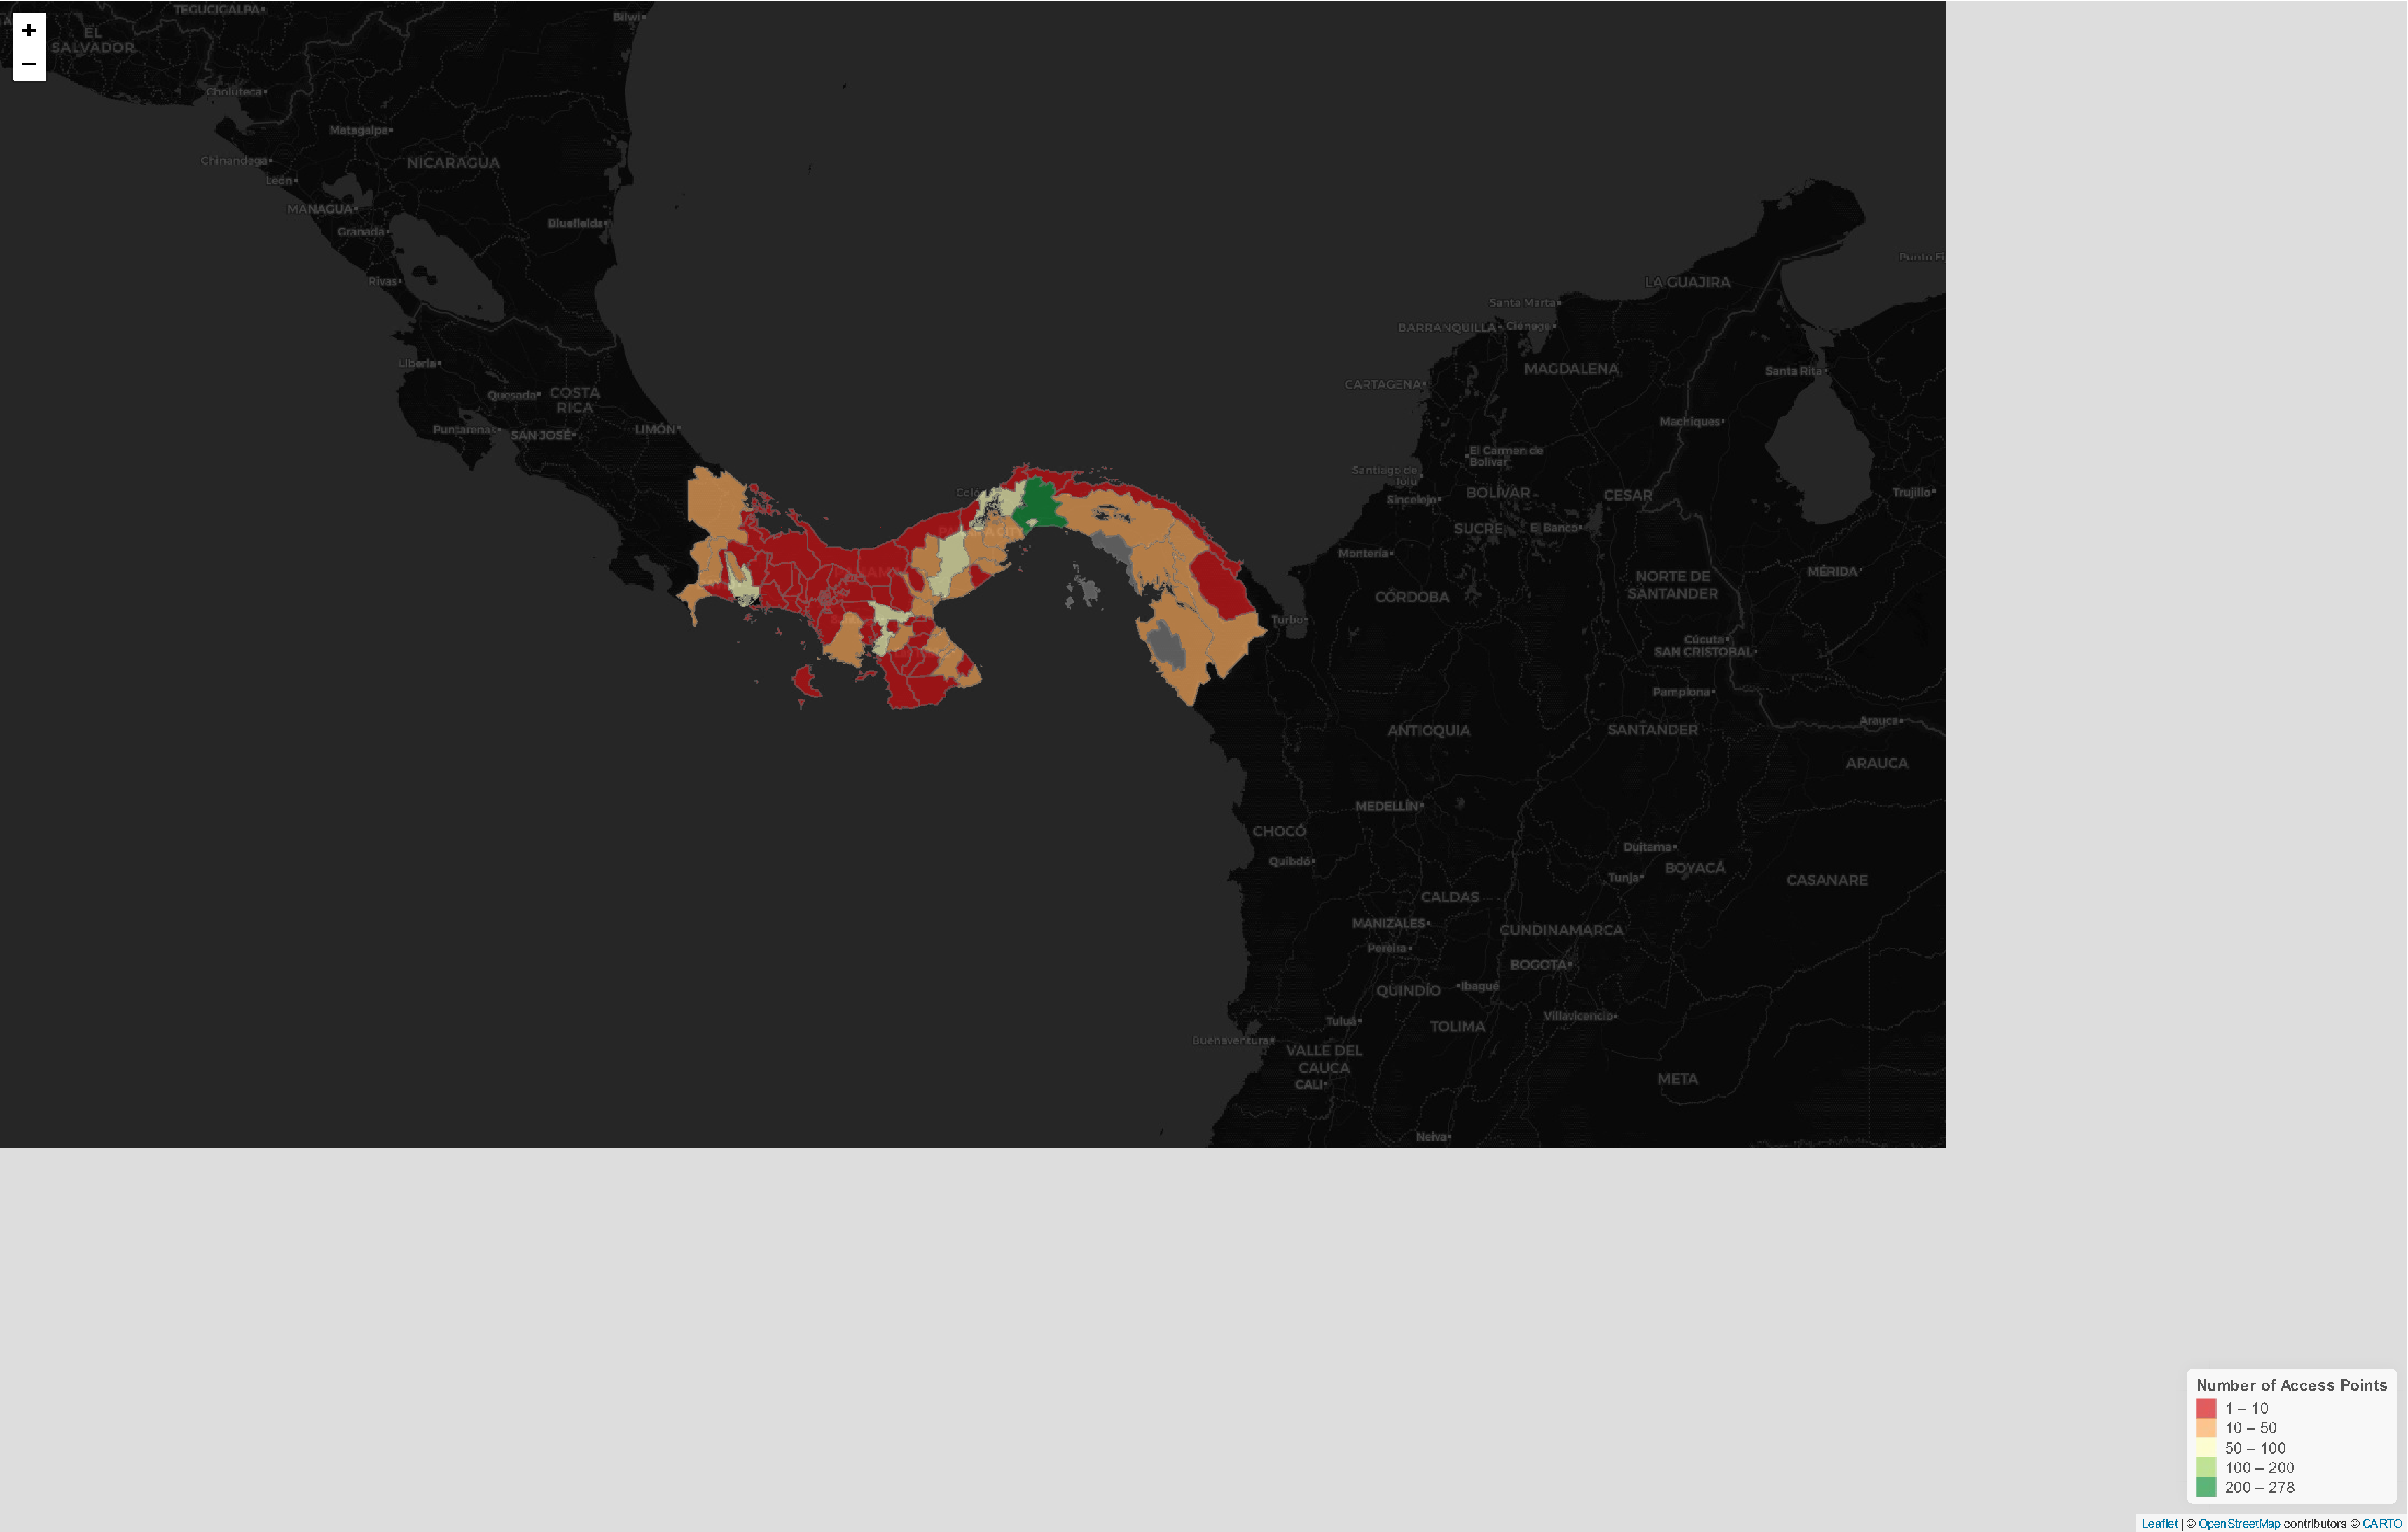
\includegraphics{index_files/figure-pdf/district-data-access-points-1.pdf}

\textbf{Panama Highway Map}

Highways represent economic development, as they try to bridge different
disitrcts across the country. Our hypothesis here is that, access points
will be located, around districts where we can see an intersection with
the Panamerican Highway. It is worth noting that this highway goes
across the complete country form west to east, mostly located on the
pacific side of the country, where Panama City is.

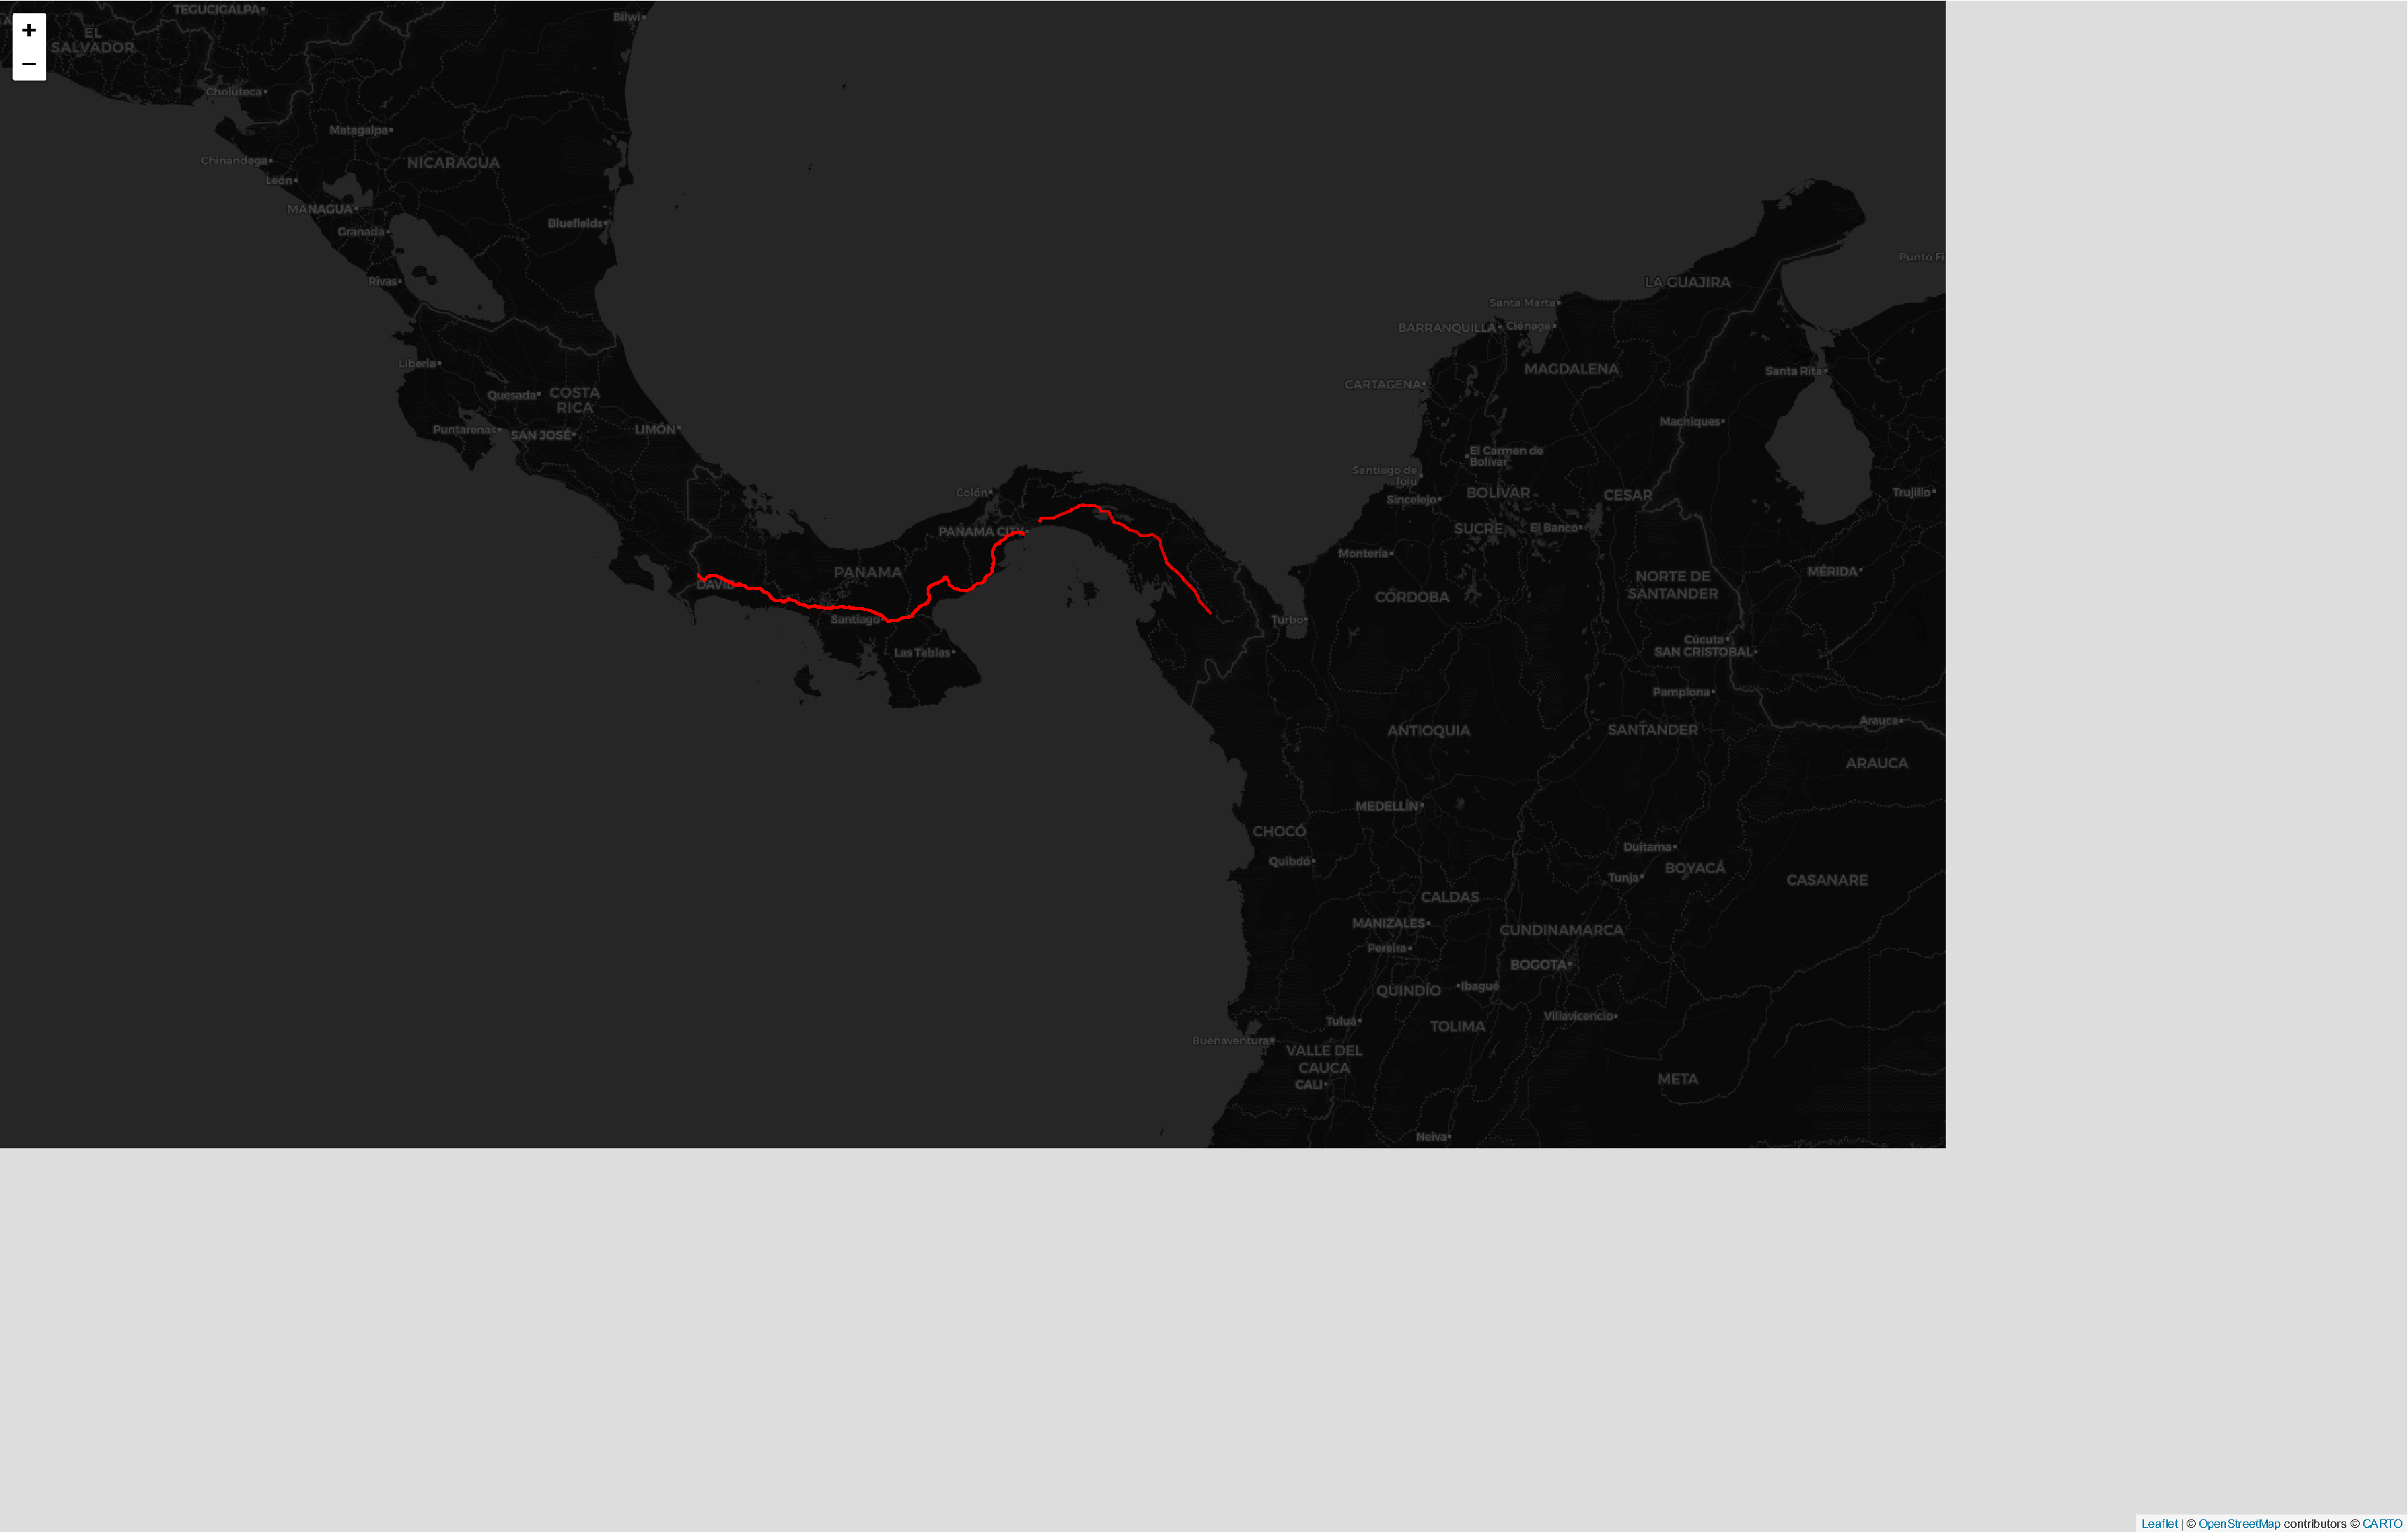
\includegraphics{index_files/figure-pdf/panama-highway-1.pdf}

\textbf{Public Schools Map}

This map shows, clustered, every school in the country. There are 9
types of classifications on the school system: - COIF - Cefacei - IPHE -
Kinder - Parvulario - Primaria Oficial - Privada - Secundaria -
Universidad

\textbf{Which Districts are Intersected by the Panamerican Highway?}

Below we find, which are the districts that intersect with the
Panamerican Highway. As confirmed by the above analysis, the districts
with the higher population densities and with the higher amount of
access points installed, are more likely to be intersected by it. This
is a causal effect of infrastructure development, as highways are more
likely to be equiped with better structures to implement different
services such as telecommunications.

\subsection{Moran's I}\label{morans-i}

\textbf{Access Points Moran's I}

We know that the scale runs from -1 (perfect dispersion) to +1 (perfect
clustering). Our result is \textbf{0.229}, which indicates positive
spatial correlation meaning that districts with similar number of access
points (higher or lower) tend to cluster together. With our p-statistic,
we can reject the null hypothesis of random spatial distribution. This
means that access points are not positioned randomly but rather
logically.

\textbf{Access Points vs Schools and Access Points vs Density Moran's I}

We know that the scale runs from -1 (perfect dispersion) to +1 (perfect
clustering). Our result is \textbf{0.229}, which indicates positive
spatial correlation meaning

\phantomsection\label{refs}
\begin{CSLReferences}{1}{0}
\bibitem[\citeproctext]{ref-berger_myanmars_2021}
Berger, Miriam. 2021. {``Myanmar's Military Built a New Capital as a
Haven for Power. {Other} Countries Have Tried That, Too.''}
\emph{Washington Post}, February.
\url{https://www.washingtonpost.com/world/2021/02/06/myanmars-military-built-new-capital-haven-power-other-countries-have-tried-that-too/}.

\bibitem[\citeproctext]{ref-campante_capital_2019}
Campante, Filipe R., Quoc-Anh Do, and Bernardo Guimaraes. 2019.
{``Capital {Cities}, {Conflict}, and {Misgovernance}.''} \emph{American
Economic Journal: Applied Economics} 11 (3): 298--337.
\url{https://doi.org/10.1257/app.20170111}.

\bibitem[\citeproctext]{ref-sackur_equatorial_2012}
Sackur, Stephen. 2012. {``Equatorial {Guinea}: {Obiang}'s Future
Capital, {Oyala}.''} \emph{BBC News}, December.
\url{https://www.bbc.com/news/magazine-20731448}.

\end{CSLReferences}



\end{document}
